\documentclass[a4paper, 10.5pt, oneside, openany, uplatex]{jsarticle}

\author{山内 仁喬}
% 余白の設定.
% 参考文献:Latex2e 美文書作成入門, 14.3ページレイアウトの変更

% 行長の変更
\setlength{\textwidth}{40zw}           %全角40文字分

% 行間を制御するコマンド
\renewcommand{\baselinestretch}{0.9}

% 左マージンを変更
\setlength{\oddsidemargin}{25truemm}   % 左余白
\addtolength{\oddsidemargin}{-1truein} % 左位置デフォルトから-1inch

% 上マージンを変更
\setlength{\topmargin}{15truemm}       % 上余白
\addtolength{\topmargin}{-1truein}     % 上位置デフォルトから-1inch

% 本文領域の縦横の長さ変更
\setlength{\textheight}{242truemm}     % テキスト高さ: 297-(25+30)=242mm
\setlength{\textwidth}{160truemm}      % テキスト幅:  210-(25+25)=160mm
\setlength{\fullwidth}{\textwidth}     % ページ全体の幅


% 図・表の個数などの設定.
%% 図・表を入りやすさを制御するパラメーター
\setcounter{topnumber}{4}
\setcounter{bottomnumber}{4}
\setcounter{totalnumber}{4}
\setcounter{dbltopnumber}{3}
\setcounter{tocdepth}{1} % 項レベルまで目次に反映させるコマンド.
\renewcommand{\topfraction}{.95}
\renewcommand{\bottomfraction}{.90}
\renewcommand{\textfraction}{.05}
\renewcommand{\floatpagefraction}{.95}

% 使用するパッケージを記述.
\usepackage{amsmath} % 複雑な数式を使うときに便利
\usepackage{dcolumn}
\usepackage{color}
\usepackage{tabularx, dcolumn}
\usepackage{bm} % 数式環境内で太字を使うときに便利.
\usepackage{subcaption}  % 関連した複数の図を並べる時に使う
\usepackage[dvipdfmx]{graphicx} % 画像を挿入したり,テキストや図の拡大縮小・回転を行う.
\usepackage{verbatim} % 入力どおりの出力を行う.
\usepackage{makeidx} % 索引を作成できる.
\usepackage{dcolumn} % 表の数値を小数点で桁を揃える.
\usepackage{lscape} % 図表を90度横に倒して配置する.
\usepackage{setspace} % 行間調整.

\def\mbf#1{\mbox{\boldmath ${#1}$}}

% \newcolumntype{d}{D{+}{\,\pm\,}{4,5}}
% \newcolumntype{i}{D{+}{\,\pm\,}{-1}}
% \newcolumntype{.}{D{.}{.}{6,3}}

\begin{document}


\title{分子モデリング}
\maketitle

\section{濃度換算}
分子モデリングをする際には, 実験で使用されたイオン濃度をシミュレーションでも再現することが多い. 
その際に, 何個のイオン原子を含めるかを計算する必要がある. 
この章では, 濃度換算についてまとめる. 


\subsection{モル濃度}

モル濃度の定義は以下の通りである. 
\begin{itemize}
    \item 単位体積の溶液中の溶質の物質量
    \item SI単位系で $\mathrm{mol}/\mathrm{m}^{3}$
\end{itemize}

モル濃度をモーラー($\mathrm{M} = \mathrm{mol}/\mathrm{L}$)へ単位変換は以下の通りである. 
\begin{align}
    \mathrm{mol}/\mathrm{m}^{3} =&
    10^{-3} ~\mathrm{mol} / \mathrm{dm}^{3} \\ =&
    10^{-3} ~\mathrm{mol} / \mathrm{L} \\ =&
    10^{-3} ~\mathrm{M} \\ =&
    1 ~\mathrm{mM}
\end{align}


\subsubsection{例1: $2.00~\mathrm{mol/L}$のNaCl水溶液を100~mL調整する}
NaClのモル濃度は58.4~g/molである. 
必要なNaClは
\begin{align}
    &2.00~(\mathrm{mol/L}) \times 58.4~(\mathrm{g/mol}) = 116.8~(\mathrm{g/L}) \\
    &116.8~(\mathrm{g/L}) = 0.1168~(\mathrm{g/}10^{-3}\mathrm{L}) = 0.1168~(\mathrm{g/mL}) \\
    &0.1168~(\mathrm{g/mL}) \times 100~(\mathrm{mL}) = 11.7 (\mathrm{g})
\end{align}
故に11.7~gのNaClを100mLになるまで水を足せば, 2.00~mol/LのNaCl水溶液が完成する. 


\subsubsection{例2: NaCl水溶液におけるNaClの質量分率, 体積, モル濃度の計算}

100~mLの水に11.6~gのNaClが溶解している. 溶液の密度は1.07~g/mL, 
水の密度を1.00~g/mLとする. この時, NaClの質量分率は
\begin{equation}
    \frac{11.6~(\mathrm{g})}{11.6~(\mathrm{g}) + 100~(\mathrm{g})}
    \times
    100 \%
    =
    10.5 \%
\end{equation}
一方で水(H$_2$O)の質量分率は
\begin{equation}
    \frac{100~(\mathrm{g})}{11.6~(\mathrm{g}) + 100~(\mathrm{g})}
    \times
    100 \%
    =
    89.6 \%
\end{equation}
である. 溶液の密度から溶液の体積は, 
\begin{equation}
    \frac{11.6~(\mathrm{g}) + 100~(\mathrm{g})}{1.07~(\mathrm{g/mL})}
    =
    104~(\mathrm{mL})
\end{equation}
NaClのモル濃度は
\begin{equation}
    11.6~(\mathrm{g}) \times
    \frac{1}{58.4~(\mathrm{g/mol})} \times
    \frac{1}{104~(\mathrm{mL})} \times
    1000 =
    1.91~\mathrm{M}
\end{equation}


\subsubsection{例3: 水溶液に含まれているイオンの数を換算する}

一辺100~{\AA}の箱にNaClが150~mM = 150 mol/m$^3$入っているとする. 
この時に, NaClがいくつ含まれているかを数える. 
まず体積をSI単位系で表す. 
\begin{equation}
    100~\mathrm{\AA} =
    100 \times 10^{-10}~\mathrm{m} =
    10^{-8}~\mathrm{m}
\end{equation}
だから, 
\begin{equation}
    (100~\mathrm{\AA})^3 =
    (10^{-8}~\mathrm{m})^3 =
    10^{-24}~\mathrm{m}^3
\end{equation}
150 mol/m$^3$の濃度の時, 1立方メートルあたりに含まれるNaClのイオンの数は, 
\begin{align}
    150 ~(\mathrm{mol/}\mathrm{m}^3) &=
    150 \times 6.0 \times 10^{23} ~(\mathrm{m}^{-3}) \\ &=
    900 \times 10^{23}  ~(\mathrm{m}^{-3}) \\ &=
    9 \times 10^{25} ~(\mathrm{m}^{-3})
\end{align}
したがって, 一辺が100~{\AA}の箱に含まれるNaClの数は, 
\begin{equation}
    9 \times 10^{25}~(\mathrm{m}^{-3}) \times 10^{-24} ~(\mathrm{m}^3)
    = 90
\end{equation}
と計算される. つまり, 90個のNaClが含まれている. 


\subsubsection{例4: 体積が$V$~({\AA}$^3$)の箱にモル濃度$x$~mMのNaClを入れる}

単位をmMからmol/m$^3$に変換すると, 
\begin{equation}
    x~(\mathrm{mM}) = x ~(\mathrm{mol/m}^{3})
\end{equation}
体積の単位をSI単位系に直すと, 
\begin{equation}
    V~(\mathrm{\AA}^{3}) =
    V \times 10^{-30} ~(\mathrm{m}^3)
\end{equation}
したがって, 
\begin{align}
    x~(\mathrm{mM}) &=
    x~(\mathrm{mol/m}^3) \\ &=
    x \times 6.022 \times 10^{23} ~(\mathrm{mol}^{-1})(\mathrm{mol/m}^3) \\ &=
    x \times 6.022 \times 10^{23} ~(\mathrm{m}^{-3}) \\ &=
    6.022 x \times 10^{23} ~(\mathrm{m}^{-3})
\end{align}

よって, 体積が$V$~({\AA}$^3$)の箱に含まれるイオンの数は, 
\begin{align}
    6.022 x \times 10^{23} \times V \times 10^{-30} =
    6.022 x V \times 10^{-7} (\mathrm{個})
\end{align}
と計算される. 

\clearpage
\section{水の初期配置について}
常温常圧における水の密度に合わせて水を配置するには, どのような間隔で並べればいいかを考える. 
水の質量, 常温常圧での密度は
\begin{itemize}
    \item 水の質量 = $18~(\mathrm{g/mol})$
    \item 水の密度 = $998.233~(\mathrm{kg/m}^3) \simeq 1.0~(\mathrm{g/cm}^3)$
    \item アボガドロ定数 = $6.02214086 \times 10^{23} ~(\mathrm{mol}^{-1})$
\end{itemize}
である. 
$1~\mathrm{cm} = 1.0 \times 10^{8}~{\mathrm{\AA}}$であるので, 
\begin{align}
    1.0~(\mathrm{g/cm}^{3}) &=
    \frac{6.02214086 \times 10^{23}}{18} ~(\mathrm{cm}^{-3}) \\ &=
    \frac{6.02214086 \times 10^{23}}{18} \times \frac{1}{10^{24}}
    ~(\mathrm{\AA}^{-3}) \\ &=
    0.334 \times \frac{1}{10} ~(\mathrm{\AA}^{-3}) \\ &=
    0.0334 ~(\mathrm{\AA}^{-3})
\end{align}
すなわち, 1~{\AA}$^3$に0.0334個の水分子が存在するような密度であるので, 1~{\AA}に0.3220個の間隔で水分子を置けばよいという計算となる. 
よって, 3.104~{\AA}に1個の水を置けば良い. 


\section{一般化螺旋集合 (GSS: Generalized Spiral Set)}
ミセルの初期構造を配置するなど, 任意の点数を球面上にできるだけ等間隔にプロットするためのアルゴリズムを考える. 
これを実現する一つの方法として, 螺旋を球面状に射影することが挙げられる. 
このような点の集合を一般化螺旋集合という. 

\subsection{アルゴリズム}
区間$[-1,~1]$を$(N-1)$等分した離散パラメータ$h$は自然数$0\le k \le N-1$を用いれば, 
\begin{equation}
    h_{k} = -1 + 2 \frac{k}{N-1}
\end{equation}
と書くことができる. 
一般化螺旋集合は以下のような漸化式で表される偏角を持つような点の集合である. 
\begin{align}
    \theta_{k} &= \arccos(h_{k}) \\
    \phi_{0} &= 0 \\
    \phi_{k+1} &= \phi_{k} + \frac{3.6}{\sqrt{N}} \frac{1}{\sqrt{1-h_{k^{2}}}}
\end{align}
$h_{k} = \pm 1$, つまり$k=0,~N-1$のとき$\phi_{k+1}$が発散してしまうのに注意. 



\clearpage

\section{水のモデル}


%\subsection{Sub section}

% \subsubsection{Sub sub section}
% \begin{figure}
%  \begin{center}
%   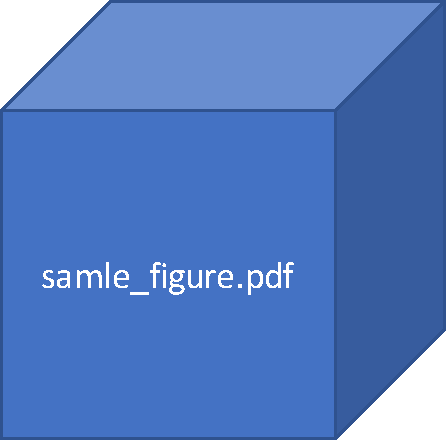
\includegraphics[width=0.5\hsize]{../figure/sample/sample_figure.pdf}
%   \caption{This is caption of sample figure.}
%   \label{Fig:Sample}
%  \end{center}
% \end{figure}

% \paragraph{Paragraph}

% \bibliographystyle{junsrt}
% \bibliography{}
\end{document}

